% BPPB submission draft
% Target journal: Biophysics and Physicobiology (BPPB), Biophysical Society of Japan
% Article type: Regular Article
% Local template base: HenriquesLab bioRxiv LaTeX class
% NOTE: swap to the official BPPB LaTeX template for final production (see AUTHOR_GUIDELINES.md).

\documentclass[times, twoside]{zHenriquesLab-StyleBioRxiv}

\usepackage{tikz}
\usetikzlibrary{positioning,arrows.meta,fit,backgrounds,shapes.geometric,calc}

% ===== BPPB DRAFT SETTINGS =====
\graphicspath{{figures/}}

% Restore first-line paragraph indentation (class sets \parindent=0pt)
\setlength{\parindent}{1em}

% Lead author for running footer
\leadauthor{Murakami}

\begin{document}

% ===== TITLE =====
\title{Simulation-informed transfer learning improves low-data nanobody thermal stability prediction}
\shorttitle{Simulation-informed Tm prediction}

% ===== AUTHORS =====
% Use letters for affiliations, numbers for equal authorship, \Letter for corresponding
\author[2]{Taihei Murakami\textsuperscript{\textdagger}}
\author[2]{Kentaro Sasaki\textsuperscript{\textdagger}}
\author[2]{Soichiro Oda}
\author[2]{Kazuma Okada}
\author[1,2]{Yasuhiro Matsunaga\textsuperscript{*}\thanks{ORCID: \href{https://orcid.org/0000-0003-2872-3908}{0000-0003-2872-3908}}}

\affil[1]{RIKEN Center for Computational Science, Kobe, Japan}
\affil[2]{Saitama University, Saitama, Japan}

\maketitle
\begin{center}
\footnotesize \textsuperscript{\textdagger}These authors contributed equally to this work.
\end{center}

% ===== BPPB MAIN TEXT =====
% SECTION_ORDER: introduction -> methods -> combined results and discussion -> conclusion
% Front matter (abstract, significance, keywords) precedes; declarations follow before References.
% abstract.tex

%TC:break Abstract
\begin{abstract}
Thermal stability limits how far a nanobody can be engineered, yet experimental
melting-temperature (Tm) measurements are scarce. Simulations and physics-based
calculations can label far more sequence variants, but they report quantities
related to Tm rather than Tm itself. We tested these labels as auxiliary supervision
for low-data Tm prediction, with model selection tied only to experimental Tm. On a public benchmark of 57 training, 114 validation, and 396
held-out test sequences, we trained multi-task models in which a Tm predictor
shared a protein-language-model representation with one computational source
task at a time. The source tasks ranged from mutation free energies and
structure-based mutation scores to Rosetta scores for language-model-proposed
variants and molecular-dynamics (MD) trajectory summaries. Alchemical free-energy perturbation (FEP) helped most. It lowered
held-out Tm mean absolute error from 6.61 to 6.26$^\circ$C, a consistent paired
gain of 0.35$^\circ$C (90\% confidence interval, 0.24--0.46$^\circ$C). Enlarging
the ESM2 encoder did not reproduce this gain, and an MD-derived Q-value did not
deliver it at all. Rosetta-scored proposal sets also worked as source labels,
but their edge over random variants stayed within noise. The value of a
computational label therefore depends on whether its physical meaning carries
over to the experimental endpoint, not on how many labels it supplies.
\end{abstract}
%TC:break main

\begin{keywords}
nanobody thermostability | melting temperature | simulation-to-real transfer learning | protein language model | free energy perturbation
\end{keywords}

\begin{corrauthor}
Yasuhiro Matsunaga, ymatsunaga\at riken.jp
\end{corrauthor}

% introduction.tex

\section*{Introduction}

Machine learning can screen molecular designs before experimental testing, but
its usefulness is limited by the labels available for training. In materials
informatics, this bottleneck has motivated simulation-to-real (Sim2Real)
learning, in which models are trained with large computational databases from
first-principles calculations, quantum chemistry, or molecular dynamics, then
adapted to smaller experimental data sets
\citep{Yamada2019Predicting,Aoki2023Multitask,Minami2025Scaling}. In some
polymer and inorganic-material settings, transfer error decreases as the
computational database grows, providing a practical test of whether additional
simulation is worth generating \citep{Minami2025Scaling}. That test is needed
because simulation data are not automatically useful. Model assumptions, finite
sampling, and domain gaps can separate a computed label from the experimental
property it is meant to support.

Protein engineering has the same label bottleneck, but the relation between
computational and experimental labels is often less direct. Experimental measurements are sparse, whereas
simulations and structure-based calculations can label many designed or mutated
sequences. Those computed labels, however, rarely measure the target phenotype
itself. For thermal stability, the experimental target may be the melting
temperature (Tm), the assay-dependent temperature at which folded and unfolded
populations are balanced. The available computed quantity may instead be a
mutation-level free-energy change ($\Delta\Delta G$), a structure-based stability
score, or a molecular-dynamics trajectory summary. Such labels are physically
related to stability, but they are not interchangeable with Tm. The central
mismatch motivates a direct test of which computed quantities transfer to
experimental Tm prediction.

We study this question for nanobodies, single-domain VHH antibodies that are
small, modular, and useful as engineered binders
\citep{Muyldermans2013Nanobodies,Alexander2024Discovery}. Their practical use in
expression, storage, and formulation depends on thermal stability
\citep{Kunz2018-qt,Mezzasalma2007-ci,Kumar2000-te}, but measuring or simulating
that stability directly is costly
\citep{Bekker2019Thermal,Higashida2021-lt,Mohseni2019-lx,Tomimoto2023-ww}.
Protein language models (PLMs) such as ESM2 provide a natural starting point
because they learn sequence representations from large protein corpora
\citep{Rives2021Biological,Lin2023Evolutionary,Hayes2025-pd}, and several recent
methods use such representations for Tm prediction
\citep{Blaabjerg2023Rapid,Li2023DeepTM,Alvarez2024TEMPRO,Savojardo2024-tv,Ramon2025-oy,Mao2026-yf}.
High-throughput stability assays are also changing the field. Tsuboyama et al.
measured folding stability for roughly 776{,}000 natural and designed protein
domains by cDNA-display proteolysis \citep{Tsuboyama2023MegaScale}. Yet those
data do not remove the need for nanobody-specific target supervision. The
mega-scale domains are 40 to 72 residues long, whereas VHH domains are longer, and
models fine-tuned on such data transfer less well to 177 to 501-residue proteins
than to small domains \citep{Chu2024EsmTherm}. For nanobody Tm prediction,
target-specific data and target-centered validation remain essential
\citep{ValdesTresanco2023NbThermo,Zhang2025NbBench,Schmirler2024FineTuning}.

Here, we test whether computed stability labels can supply useful supervision
when experimental nanobody Tm labels are scarce. We treat Tm prediction as the
target task and each computed label as a computational task that shares an ESM2-based
sequence representation \citep{Lin2023Evolutionary}. The computational labels include
mutation free energies from alchemical free-energy perturbation (FEP), Rosetta
mutation scores, ThermoMPNN stability scores, Rosetta scores on variants
proposed by ESM2 or sampled at random, and an MD-derived native-contact stability
label computed either over the same mutation scans used for FEP or, as a control,
over a diverse panel of nanobodies. To keep the comparison target-centered and
fair across very different labels, every source is tuned independently and selected
on experimental Tm validation data, and every final claim is evaluated on the same
held-out experimental Tm test set with paired error statistics.

\begin{figure*}[t]
\centering
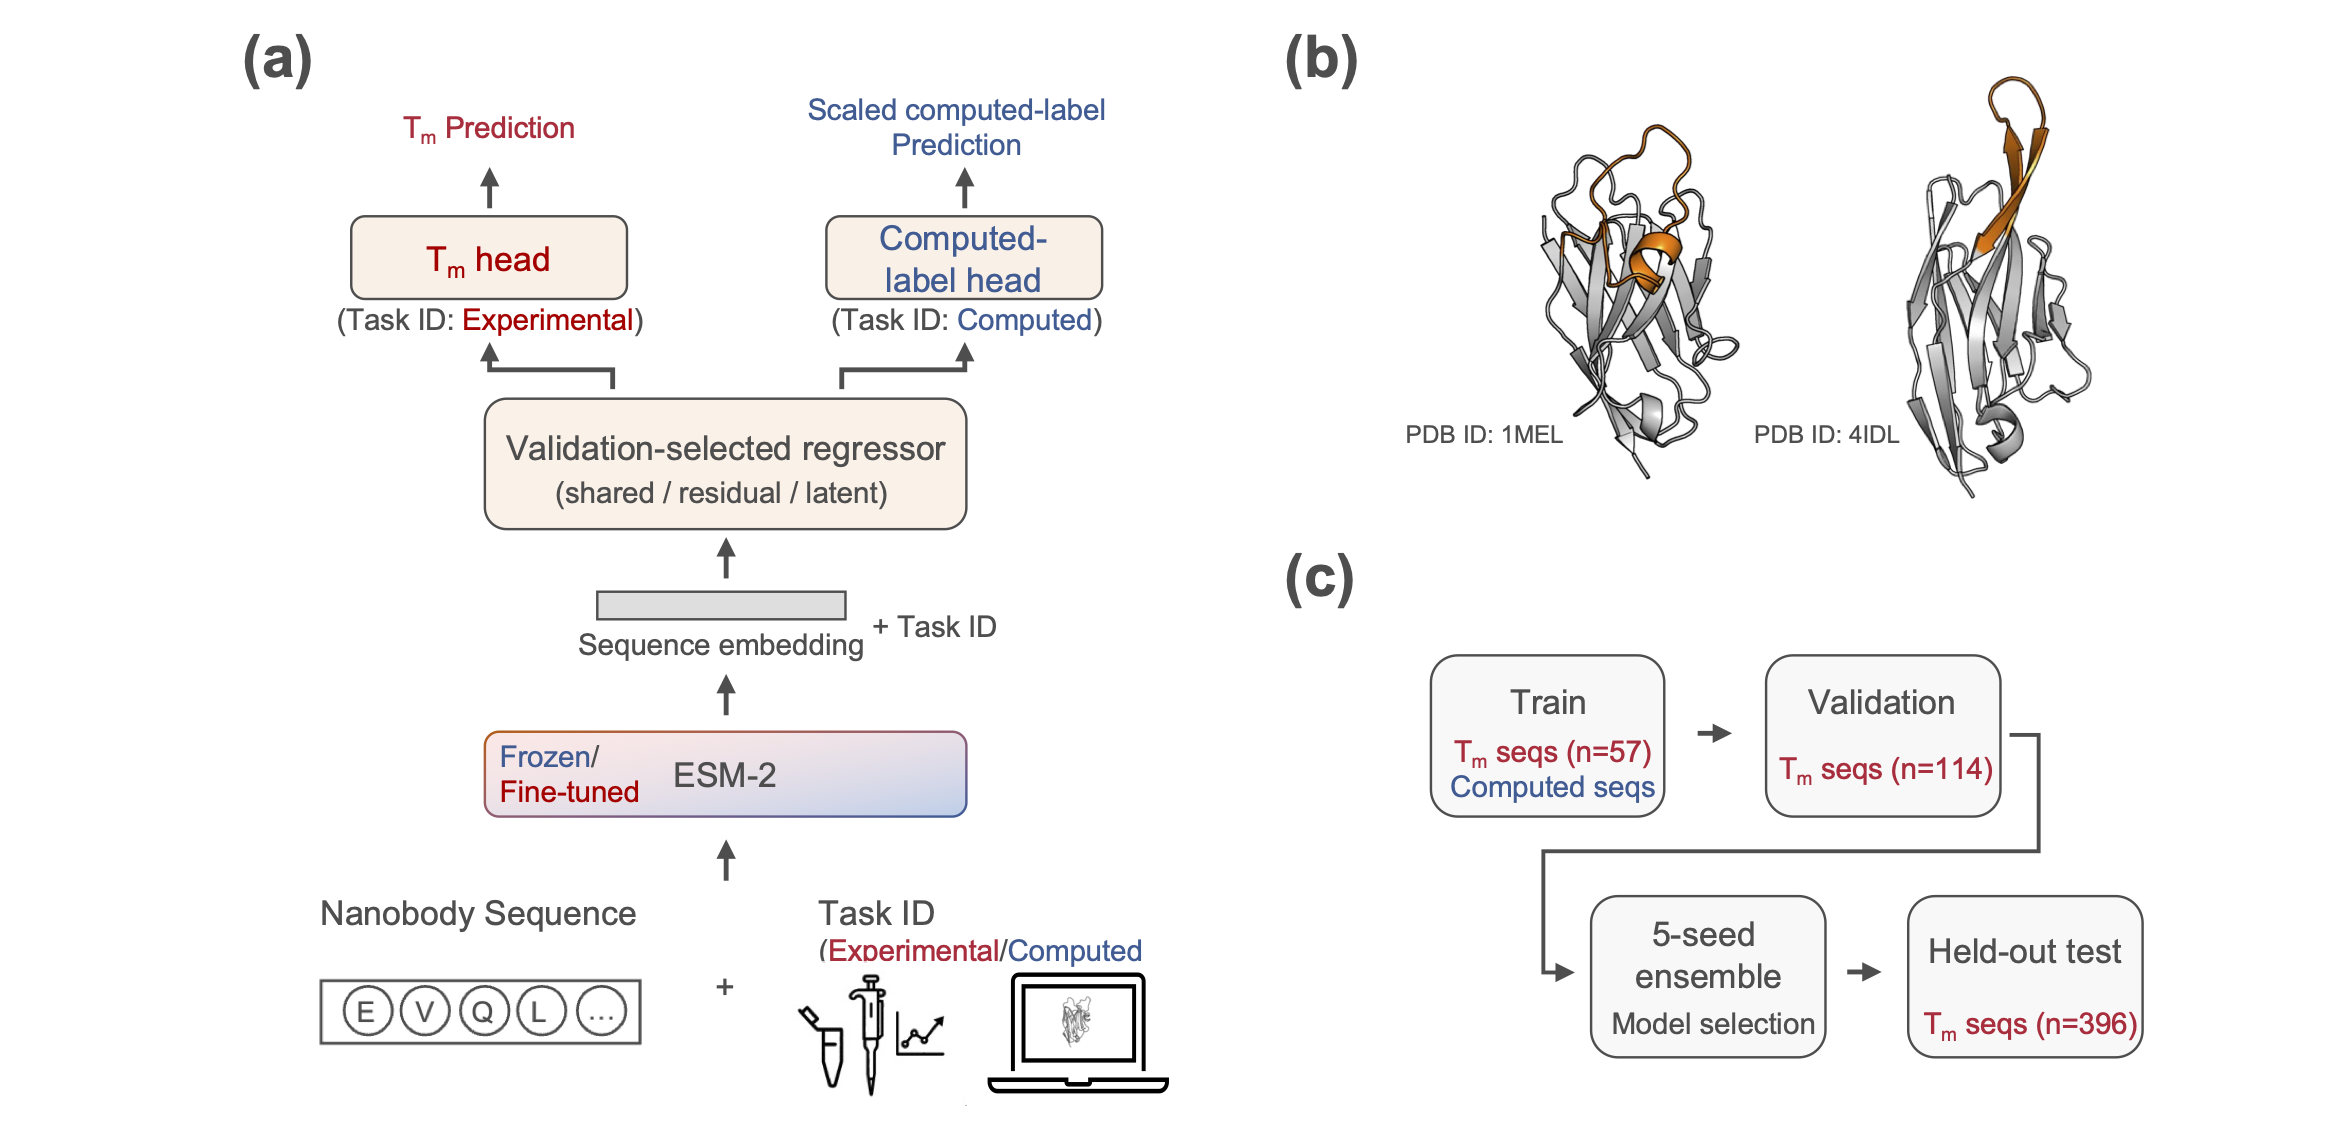
\includegraphics[width=0.66\textwidth]{figure_1_concept_protocol_v2}
\caption{\textbf{Multi-task transfer-learning architecture for using simulation
data in experimental Tm prediction.}
Experimental sequence data (left) and computational sequence data (right) are
encoded by a shared ESM2 protein language model into per-sequence embeddings.
The embeddings pass through a shared multilayer perceptron and then split into
two task-specific heads: a Tm head that predicts the experimental melting
temperature, and a computational head that predicts the computational scores
(mutation $\Delta\Delta G$ values or an MD-derived Q-value). Only the
experimental Tm head defines the final objective, while the computational head lets the
simulation-derived labels reshape the shared representation during training.
Flame and snowflake icons mark trainable and frozen parameters, respectively;
the ESM2 encoder is either fine-tuned (hot) or kept frozen depending on the
configuration.}
\label{fig:learning_framework}
\end{figure*}

The results are organized by two design axes. First, \emph{data design}: the same
MD native-contact observable does not improve Tm when computed over a
diverse-nanobody screen, but does when computed on the FEP-matched mutation scans,
where it matches FEP with a frozen encoder --- so matching the auxiliary source's
sequence design to the target, not the choice of dynamical quantity, is what lets
an MD label transfer.
Second, the \emph{physical observable}: the alchemical FEP free energy improves Tm
whether the encoder is frozen or fine-tuned, whereas the native-contact label helps
only a frozen encoder, so the physical content of the label sets how deeply it
transfers. The other structure-based scores are weak or null under the same
tuning. These results extend the Sim2Real argument to a protein-engineering setting
in which the computational and experimental labels differ in physical meaning, and
turn "run more simulation" into two concrete design choices --- matched data design
and a transferable observable --- that decide whether computed data help.

% methods.tex

\section*{Methods}

% TODO: Key methodologies
\blindtext

\subsection*{Data Collection}
% TODO: Data collection methods
\blindtext

\subsection*{Analysis}
% TODO: Analysis methods
\blindtext

% results.tex

\section*{Results}

\subsection*{A target-centered framework for using simulation labels in Tm prediction}

The target task was nanobody melting-temperature (Tm) regression from
amino-acid sequence. Computational labels were treated as auxiliary prediction
tasks, not as stand-ins for experimental Tm. Each model used the pretrained
protein sequence model ESM2 to turn a sequence into a learned representation
that a Tm head and an auxiliary head shared, so the auxiliary task could reshape
the representation while the final objective stayed anchored to experimental Tm
(Fig.~\ref{fig:learning_framework}).

We used the benchmark split as a deliberately low-data target setting, with 57
experimental Tm labels for training, 114 for validation, and 396 for held-out
testing. To keep the comparison fair across very different auxiliary labels,
each source was tuned independently: for every source and every encoder regime we
searched the model architecture, the auxiliary-head coupling, and the learning
rate, dropout, and weight decay, selecting on the experimental Tm validation set
alone. Only the selected configuration was then evaluated on the held-out Tm test
set, and improvements were measured as paired differences in absolute error on the
same test examples. This target-centered protocol guards against a trap specific
to simulation-to-experiment learning: an auxiliary task can be learnable and
physically sensible yet do nothing for the experimental phenotype. Under this
protocol the tuned Tm-only baselines were 7.23$^\circ$C MAE with a frozen encoder
and 6.55$^\circ$C MAE with a fine-tuned (hot) encoder. Two design axes organize the
results: whether a simulation label transfers at all is set by its \emph{data
design} (Fig.~\ref{fig:data_design}), and how deeply it transfers is set by its
\emph{physical observable} (Fig.~\ref{fig:physical_observable}).

\subsection*{Data design: matching the sequence scan makes an MD label transfer}

With each source tuned to the same Tm endpoint, two all-atom labels clearly
transferred: the FEP mutation free energy and --- new to this work --- an MD
native-contact stability label computed on the \emph{same} 1MEL and 4IDL mutation
scans used for FEP. The MD native-contact label uses one physical observable in
two different data designs, which isolates the effect of data design from the
choice of quantity. Computed over an earlier screen of diverse nanobodies, the
label did not improve Tm: its held-out error sat at or slightly above the
corresponding Tm-only reference (Fig.~\ref{fig:data_design}a, upper group).
Computed instead over the FEP-matched mutation scans --- the same scaffolds, all of
constant length --- the identical observable improved Tm and matched FEP with a
frozen encoder (Fig.~\ref{fig:data_design}a, lower group). Because the two groups
come from different training series with different absolute baselines, each is
shown against its own Tm-only reference and the two are not cross-compared
numerically.

The difference is a data-design confound, not the label arithmetic
(Fig.~\ref{fig:data_design}b). The diverse screen spans sequence lengths from 58 to
461 residues and carries a nonzero label--length correlation ($r = +0.13$), a
length signal the auxiliary task can latch onto instead of the stability signal;
the matched scans are of constant length, so no such confound exists. Referencing
each mutant's native-contact value to its wild type (a $\Delta Q$) versus using the
raw value is immaterial here, because a constant offset is absorbed by the min--max
scaling applied to every label. With the confound removed, both all-atom labels
scale below the Tm-only baseline as the number of auxiliary labels grows: with a
frozen encoder the FEP curve stays below the baseline throughout (7.13 at 20
labels to 7.01 at 320), and the matched-scan MD curve falls from above it to below
it, crossing by 320 labels (7.32 to 7.03; Fig.~\ref{fig:data_design}c). At 320
labels the matched MD label improved held-out Tm by $-0.20^\circ$C
(90\% CI $-0.34$ to $-0.05$), statistically indistinguishable from FEP in the same
regime ($-0.22^\circ$C; paired FEP-minus-MD difference $-0.03^\circ$C, 90\% CI
$-0.21$ to $+0.16$). Matching the auxiliary source's sequence design to the target
neighborhood, not the specific dynamical quantity, is what lets the MD label
transfer.

\begin{figure*}[t]
\centering
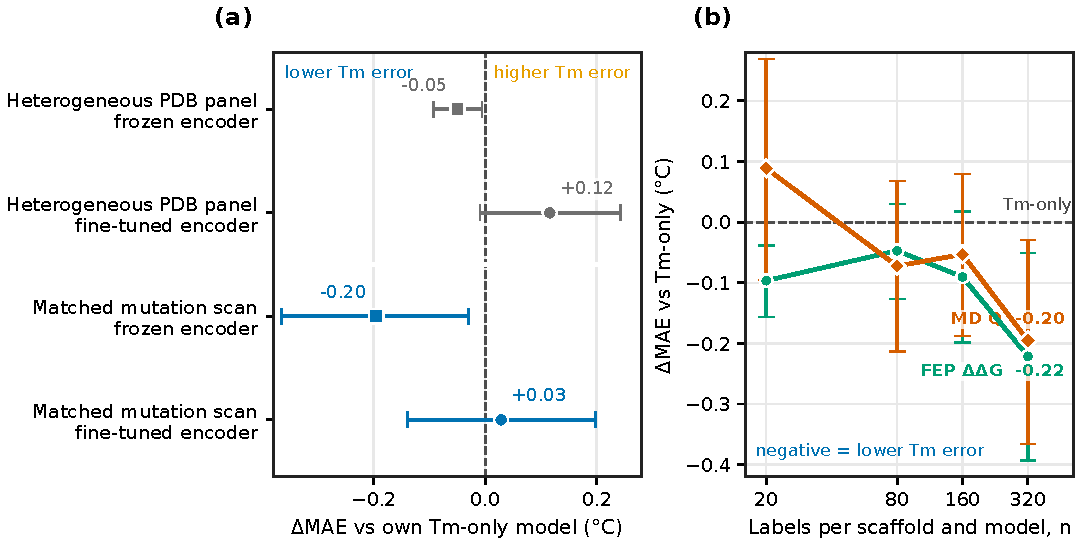
\includegraphics[width=\textwidth]{fig_outline02_data_design}
\caption{\textbf{Data-design axis: a matched mutation scan makes the MD label transfer.}
(a) Held-out test MAE for the MD native-contact label computed over a diverse
nanobody screen (upper) versus the FEP-matched 1MEL/4IDL mutation scan (lower),
each with its own Tm-only and FEP references. The two groups are from different
training series (different absolute baselines) and are not compared numerically
across groups; the point is null-versus-positive for the same observable.
(b) The confound made explicit: MD native-contact value versus sequence length.
The diverse screen has a broad length spread (58--461 residues) and a nonzero
label--length correlation ($r = +0.13$); the matched scans are constant length.
(c) Frozen-encoder label-count sweeps for FEP and the FEP-matched MD native-contact
label; the dashed line is the Tm-only frozen baseline. Both labels fall below the
baseline as labels increase, and the matched MD label crosses it by 320 labels.
Points and intervals show ensemble MAE and 90\% bootstrap intervals.}
\label{fig:data_design}
\end{figure*}

\subsection*{Physical observable: free energy transfers deeper than native contacts}

Tuned to the same endpoint, the sources formed a clear frozen-encoder hierarchy
(Fig.~\ref{fig:physical_observable}a): FEP (7.01) and the matched-scan MD label
(7.03) led, both improving on the Tm-only baseline (7.23); ThermoMPNN was a weak
third (7.09, 90\% CI crossing zero); and the Rosetta-family scores --- the plain
Rosetta mutation score and Rosetta scores on ESM2-proposed or random variant sets
--- sat at the baseline (7.23, 7.31, and 7.22). But a matched data design was
necessary, not sufficient: the two all-atom labels differed in how deeply they
transferred across encoder regimes (Fig.~\ref{fig:physical_observable}b). The FEP
free energy improved Tm whether the encoder was frozen or fine-tuned (frozen
$-0.22^\circ$C, 90\% CI $-0.36$ to $-0.08$; hot $-0.15^\circ$C, 90\% CI $-0.30$ to
$-0.01$), reaching the best held-out accuracy overall (6.40$^\circ$C MAE, hot). The
MD native-contact label improved Tm only with a frozen encoder; once the encoder
was fine-tuned it gave no net gain and, at small label counts, degraded prediction
(paired $+0.47^\circ$C at 20 labels, 90\% CI $+0.29$ to $+0.65$), recovering only
to the baseline by 320 labels. Directly, FEP beat the MD label in the hot regime
($-0.18^\circ$C paired, 90\% CI $-0.36$ to $-0.01$) while tying it when frozen.

The natural reading is that the alchemical free energy carries enough information
about the mutation's effect on stability to beneficially reshape the sequence
encoder, whereas a native-contact persistence label can usefully condition a fixed
representation but cannot steer encoder fine-tuning toward the Tm phenotype
(Fig.~\ref{fig:physical_observable}c). The physical content of the label sets the
\emph{depth} of transfer. The Rosetta-family scores fit the weaker side of this
picture: they did not robustly improve Tm in either regime. In particular the two
Rosetta-scored variant sets (ESM2-proposed and random variants) are ordinary
comparators; under tuning the ESM2-proposed set did not outperform the random set,
so we make no claim about physics-scored sequence proposals as a design loop.
Enlarging the ESM2 encoder from 8M to 35M or 650M parameters did not by itself
reproduce the FEP gain (Supplementary Fig.~4), so model capacity does not
substitute for a matched physical label.

\begin{figure*}[t]
\centering
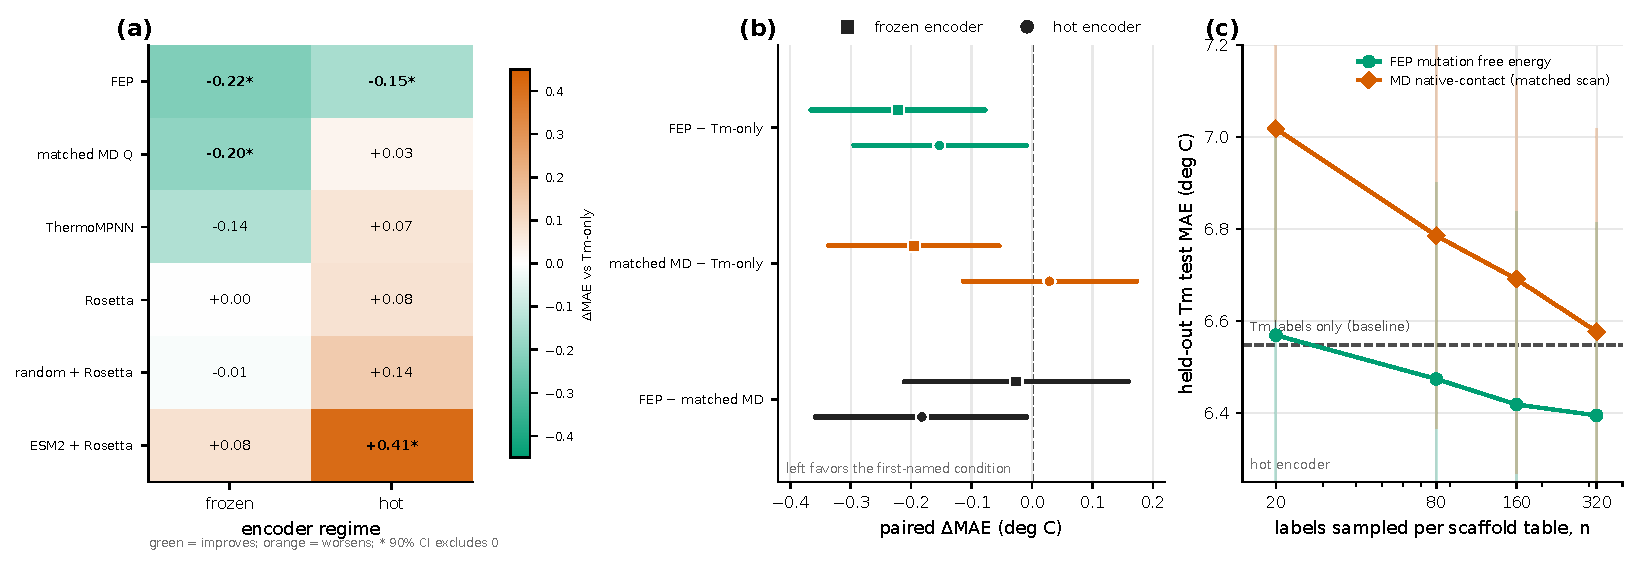
\includegraphics[width=\textwidth]{fig_outline03_physical_observable}
\caption{\textbf{Physical-observable axis: depth of transfer set by the simulated quantity.}
(a) Tuned frozen-encoder held-out test MAE for every source; the dashed line is the
Tm-only baseline. FEP and the matched-scan MD label lead; the Rosetta-family scores
sit at the baseline.
(b) Paired $\Delta$MAE versus Tm-only for FEP, the MD native-contact label, Rosetta,
and ThermoMPNN under frozen versus hot encoders; values left of zero improve on
Tm-only. FEP crosses below zero in both regimes; the MD native-contact label only
when frozen; Rosetta and ThermoMPNN sit near zero.
(c) Interpretation: the free-energy label reshapes the shared encoder (deep;
transfers frozen and hot), whereas the native-contact label only refines the fixed
trunk (shallow; helps frozen, not hot). Points and intervals show ensemble MAE and
90\% bootstrap intervals.}
\label{fig:physical_observable}
\end{figure*}

Across every label we tested, the improvements were selective rather than
additive. Two axes organize the pattern: a matched data design decides whether a
simulation label transfers at all, and the physical observable decides how deep
that transfer goes. Under both, only the FEP mutation free energy (in both
regimes) and the FEP-matched MD native-contact label (with a frozen encoder)
robustly improved low-data nanobody Tm prediction.

% conclusion.tex

\section{Conclusion}

Computed labels did not improve low-data nanobody Tm prediction uniformly.
Among two independently developed MD data sets, matched mutation scans showed a
larger reduction with the frozen encoder than the heterogeneous
structure panel, although differences in their protocols prevent attribution to
sequence selection alone. FEP had the lowest test MAE with both
frozen and fine-tuned ESM2; its 95\% interval excluded zero only with the frozen
encoder. The comparisons did not show a simple relation between label count and
Tm error. When calculations are intended to support Tm prediction, both the
variants and the physical property should be considered from the start.

One extension is to repeat matched scans across more nanobody structures and
select new calculations adaptively. Reinforcement learning could support this
sequential selection, but random sampling and simpler active-learning methods
would be necessary baselines. A computed score alone should not define success:
under the present Rosetta protocol, ESM2 proposals did not yield lower Tm
prediction error than random variants. Any improvement should ultimately be
tested with new experimental Tm measurements.

% Declarations in BPPB order (Conflict of interest, Author contributions,
% Data availability, Acknowledgements); AI-use disclosure inside Acknowledgements.
% acknowledgments.tex

\begin{acknowledgements}
This work was supported by JSPS KAKENHI (Grant number: 23H03412) and JST NBDC (Grant number: JPMJND2603), and partly supported by MEXT as ``Program for Promoting Researches on the Supercomputer Fugaku'' (Development and application of large-scale simulation-based inferences for biomolecules JPMXP1020230119). Computational resources were provided by the supercomputer Fugaku at the RIKEN Center for Computational Science (Project IDs: hp230209, hp240215, hp250233).
\end{acknowledgements}

\begin{contributions}
Yasuhiro Matsunaga conceived and supervised the study, acquired funding, developed the analysis and training code, performed the analyses, interpreted the results, prepared the figures, and wrote the manuscript. Kentaro Sasaki performed computational calculations. Taihei Murakami contributed to draft writing. All authors reviewed and approved the final manuscript.
\end{contributions}

\section*{Declaration of competing interest}
Taihei Murakami is an employee of Epsilon Molecular Engineering, Inc. Yasuhiro Matsunaga is a scientific advisor of Epsilon Molecular Engineering, Inc.

\section*{Data availability}
Processed data required to reproduce the main and supplementary figures will be deposited in Zenodo at \url{ZENODO_DATA_DOI_PLACEHOLDER}. Raw simulation trajectories are large and will be made available at \url{RAW_DATA_LOCATION_OR_REQUEST_POLICY_PLACEHOLDER}.

\section*{Code availability}
Analysis, training, and figure-generation code will be available on GitHub at \url{GITHUB_REPOSITORY_URL_PLACEHOLDER}. An archival release will be deposited in Zenodo at \url{ZENODO_CODE_DOI_PLACEHOLDER}.

\section*{AI-use disclosure}
AI-assisted tools were used to support language editing, code development, and figure preparation. The authors reviewed and take responsibility for all manuscript content, analyses, and conclusions.

% ===== END BPPB MAIN TEXT =====

% ===== REFERENCES =====
\section*{References}
\bibliography{refs}

% ===== SUPPLEMENTARY MATERIALS =====
%TC:ignore
\onecolumn
\clearpage
% supplementary.tex

\section{Supplementary methods}

\subsection{Additional details for the diverse MD panel}

The diverse panel was assembled from an archived SAbDab summary and the
corresponding IMGT-renumbered structures \citep{Dunbar2014SAbDab}. For each PDB
identifier, the workflow took the first heavy-chain entry whose chain identifier
was present in the structure file. After availability checks, this deterministic
selection yielded 1143 structures with a usable sequence, topology, trajectory,
and native-contact label.

The selected heavy chain was kept as an uncapped protein at pH 7.4, solvated in
OPC water with 15~\AA{} padding and 0.15~M NaCl, and described with ff19SB
\citep{Tian2020ff19SB,Izadi2014OPC}. The 300-K branch comprised 1~ns NVT and
1~ns NPT with a 2-fs timestep. Two 1-ns restrained NVT stages at 400~K preceded
100~ns of unrestrained 400-K NVT production. Production used hydrogen-mass
repartitioning to 4~amu, a 4-fs timestep, and output every 100~ps. OpenMM used
PME electrostatics with a 1.0-nm cutoff, constraints on bonds to hydrogen, and a
Langevin middle integrator with 1~ps$^{-1}$ friction
\citep{Eastman2017OpenMM}.

The diverse-panel contact calculation used backbone heavy-atom pairs separated
by more than three residues, within 0.45~nm in the reference structure, and with
at least one atom in Asp, Glu, Gln, Asn, Arg, Lys, or His. For trajectories with
more than 300 frames, the label was averaged over the larger of the final 300
frames and the final one third of the trajectory; all frames were used for
shorter trajectories. Supplementary Fig.~S1 shows the relation between sequence
length and the resulting raw $Q$ value.

\subsection{FEP provenance and charge-change check}

The retained FEP tables contain Ala, Asp, Ile, and Gln scans. Row-level
provenance was checked against the archived scan outputs; the available Phe
scans were not included.

For charge-changing mutations in a cubic 70-\AA{} box and solvent dielectric
78, we tested an analytical periodic net-charge correction of
$0.086(\Delta q)^2$ kcal mol$^{-1}$. We applied the correction before repeating
the sign reversal, robust scaling, Yeo--Johnson transform, and min--max scaling
used for the model-facing labels (Supplementary Fig.~S2b).

\renewcommand{\thefigure}{S\arabic{figure}}

\begin{figure}[p]
\centering

\includegraphics[width=\textwidth]{supp_fig01_data_and_design}
\caption{Sequence length and native-contact $Q$ in the heterogeneous MD panel.
Hexagons show row density, and dashed lines mark the fixed sequence lengths of
the 1MEL and 4IDL matched mutation scans. The observed association is
descriptive and does not establish that length caused the transfer difference.}
\label{fig:supp_data_design}
\end{figure}

\begin{figure}[p]
\centering
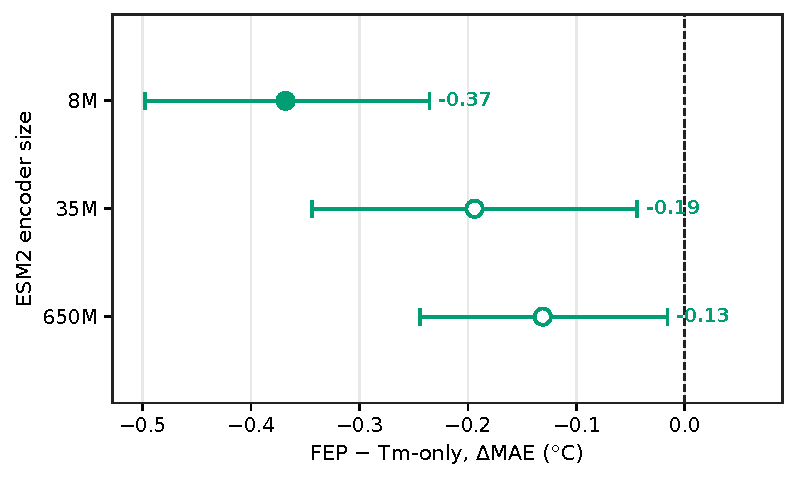
\includegraphics[width=\textwidth]{supp_fig02_transfer_controls}
\caption{Robustness controls for the FEP result.
\textbf{(a)} Paired FEP-minus-Tm-only MAE for fine-tuned ESM2 encoders. Negative
values mean lower Tm error with FEP. The 8M point is the staged-selected
five-seed model; the 35M and 650M points are exploratory fixed-configuration
ten-seed controls and were not subjected to the same search. Whiskers are
nominal 90\% paired bootstrap intervals over the 396 test proteins.
\textbf{(b)} Change in each scaled FEP label after the analytical periodic
net-charge correction at dielectric 78.}
\label{fig:supp_transfer_controls}
\end{figure}

%TC:endignore

\end{document}
